%----------------------------------------------------------------------------------------
%	Introduction to PsyToolkit CHAPTER 
%----------------------------------------------------------------------------------------
\chapterimage{ChapterCover.pdf} % Chapter heading image
\chapter{Methods for Data Collection}

\epigraph{\textit{I do not fear computers. I fear lack of them.}}{\rightline{{\rm --- \href{https://en.wikipedia.org/wiki/Isaac_Asimov}{Isaac Asimov}}}}

\minitoc
\newpage
\section{Software for Generating Experiments}
The advent of desktop-computers forever changed the landscape of research in nearly all scientific fields.  For psychological science, desktop computers have made possible new ways of probing the cognitive, emotional, and social functions of the brain. In addition to software that facilitates data management and analysis, computers can be used for flexible and precise control over many aspects (e.g.., stimuli and responses) of experimental procedures. It is their central role in the scientific process, from experimental design, to data collection, to data analysis, to typesetting a formal report of the results that makes a broad range of computing skills so critical to success in the psychological sciences. Of course, each aspect of research requires its own set of computing competencies. Here, emphasis will be placed on the design of experiments and collection of data. 

\subsection{Choosing the Right Software}
\subsubsection{Commercial Vs. Open Source}
As with any task you wish to complete on a computer, there are several commercial and \gls{open source software} options available. In the case of generating psychological experiments, all of the available options provide methods for displaying text, images, sound, and/or video as well as methods for recording responses using the keyboard, mouse, or other peripheral device like a specialized button box.  The authors/distributors of these software packages also claim to provide accurate control of experiment timing, usually to within a millisecond. 

Both the open source and the commercial options have their strong advocates. One argument is that the open-source method of developing software is far superior to commercial methods. Users of open source software have access to the source code, meaning they can enhance the program’s performance, add features, and fix errors. In fast-paced scientific fields, this can mean that open source software will likely be the first to implement the latest and greatest methods. In the event of the establishment of novel methods, those who develop commercial software (a.k.a. ``closed source software") must employ their programming team to implement the method within their software and run exhaustive testing in order to be able to provide assurance of accuracy/reliability to their customers before releasing a software update. 

The most staunch proponents of commercial software often argue that this assurance of accuracy and reliability is precisely what makes it preferable to open source software.  Another advantage of commercial software is the product support that is offered along with purchase of the software.  If you download software like PsychoPy and receive an error when you attempt to install it, or are unable get it working properly after installation, your only option is to post your question to one of the online discussion boards dedicated to PsychoPy, and hope for a response.  On the other hand, if you purchase a license to use E-prime\copyright and have trouble installing the software and/or running an experiment, you can call the company and speak to an employee who's job it is to help you solve your specific problem. Ultimately, there are costs and benefits of both commercial and open source software and selection of a specific program should, most importantly, be based on how well that software will facilitate your research agenda.

\subsubsection{Flexibility Vs. Ease of Use}
Experiment control software also varies considerably on dimensions of flexibility and ease of use. Unfortunately, these two important dimensions tend to be inversely related to one another (see Figure \ref{fig:ExpCtrlApps} in almost any programming context. The reason for this inverse relationship is computers only do \emph{exactly} what you tell them to do.  When it comes to designing an experiment, instructing the computer about the many related details such as what image should appear on the monitor, where it should appear, how long it should remain on the monitor, whether or not to record a response from participants in your experiment all can be quite complicated. 

\begin{wrapfigure}{R}{0.5\textwidth}
\begin{tcolorbox}[every float=\centering, drop shadow, title=Trade off between Flexibility and Ease of Use ,colback=WMgold,colframe=WMgreen,
  colbacktitle=WMgreen,]
  \begin{tikzpicture}[%
    filled/.style={circle,fill=WMgreen,text=white,font=\large},
    label distance=4pt]
\coordinate (O) at (0,0);
\draw (-3,-3) -- (3,-3);
\draw (-3,-3) -- (-3,3);
\node [above right, align=center,filled] at (-2,0) {More\\Programming};
\node [above right, align=center,filled] at (.5,-2.2) {More\\Point \& Click};
\node [below, align=center] at (0,-3) {Ease of Use};
\node [left, align=center, rotate=90] at (-3.3,1) {Flexibility};
  \end{tikzpicture}
  \captionof{figure}{Illustration of the trade-off between flexibility and ease of use in experiment control software}
  \label{fig:ExpCtrlApps}
 \end{tcolorbox}
 \end{wrapfigure}
 
Software that is easy to use tends be more ``point \& click", meaning that the software's author(s) have, in order to simplify the process of creating an experiment, reduced the number of instructions you are required to give to the computer by implementing a number of assumptions about how the experiment should run.  Although these assumptions effectively relieve everyday users of the burden of having to understand much of the underlying programming language, this ease of use often comes at the cost of flexibility. Finding a good balance of flexibility and ease of use is important so that novel and/or dynamic research needs can quickly be addressed but implementation of those needs does not require complete mastery of a programming language. While a complete review of the available software is beyond the scope of this chapter, software reviews do occasionally appear in the literature \citep[e.g.,~][]{stahl2006software}.

Most commercial software is available through stand-alone packages, meaning that once the software has been purchased, there are no other dependencies or packages required other than those that are already installed on your computer. Some examples of commercial software are \weblinkT{https://pstnet.com/}{E-prime\copyright}, \weblinkT{https://cedrus.com/superlab/index.htm}{SuperLab}, \weblinkT{https://www.neurobs.com/}{Presentation}, and \weblinkT{https://www.empirisoft.com/DirectRT.aspx}{DirectRT}, just to name a few. It can be quite difficult to draw direct comparisons between these different options because each one has a unique set of strengths and weaknesses and are typically designed to meet the needs of users in specific research contexts. For example, two historically popular choices are E-Prime and SuperLab, each of which offers an easy to use point \& click style interface with which simple experiments can be generated in just a few minutes. Another popular commercial option is Presentation.  Although Presentation does not have the same kind of graphic user interface (GUI) as E-prime\copyright or Presentation, the language includes a powerful set of commands for designating experimental components (e.g., images, sounds, responses etc.) and their timing (e.g., onset, offset, duration, etc.).

 A popular open-source option for the generation of experiments is \weblinkT{http://psychtoolbox.org/HomePage}{Psychtoolbox}. With years of development and a broad base of users, Psychtoolbox boasts a wide variety of powerful, well-developed routines for experimental control. However, Psychtoolbox is written in the Matlab programming language, meaning that using it requires that you have a licensed installation of Matlab. Thus, while Psychtoolbox is freely available, there is an indirect, prerequisite cost of obtaining Matlab\footnote{Note that the latest version of the Psychtoolobx is also compatible with GNU Octave, a free alternative to Matlab}. Like Presentation, Psychtoolbox lacks a GUI so even simple experiments require at least some experience with the Matlab programming language, making it difficult for new users without much programming experience.
 
Another open source option is \weblinkT{https://www.psychopy.org/}{PsychoPy}. Written in the Python programming language, itself a free alternative to programs like Matlab, PsychoPy offers an attractive balance of flexibility and ease-of-use.  PsychoPy has the full flexibility of any general purpose programming language, but also includes a user-friendly GUI with point \& click features that allow simple experiments to be generated with little to no knowledge of the Python programming language.

\subsubsection{Online Data Collection}
The ability to collect data online using experiment control software is a feature that has recently become especially popular.  In fact, most commercial \emph{and} open source software offers some kind of online option for data collection, but it is important to understand at least two of the central issues related to collecting data online, including  (1) the type of data being collected and (2) how will the data be stored.

The type of data being collected in an online experiment is an important consideration because some measures of behavior and/or parameters of a stimulus display require a degree of temporal precision that may be difficult to achieve in practice.  For example, an accurate measure of reaction time requires (1) precise measurement of the time at which a stimulus is presented to the participant (i.e., the stimulus to which participant is reacting) and (2) an accurate measure of the time at which a key or button was pressed.  These may seem trivial, but while computers only do exactly what they are told, they don't always do it exactly when they are told. 

Remember that modern computers are serial processors, managing many different tasks such as checking your email inbox, running virus protection software, monitoring internet traffic, etc., all while also running your experiment. Each of these tasks uses some of a limited set of resources on the computer. When the program you are using instructs the computer to display an image or play a sound, the expectation is that it will happen immediately, but this is almost never the case. Instead, the time between the instruction to present a stimulus and the appearance of that stimulus to the participant depends on a variety of factors like the amount of available resources at that moment, the priority assigned to your experimental task by the computer's CPU relative to other ongoing computer functions, characteristics of the computer's video and/or audio cards, and other computer hardware and software settings.  There is also uncertainty in the measurement of key/button press responses.  Computers only "check" the status (i.e., up/down) of keys and buttons at designated intervals; typically 125 times per second or every 8 milliseconds.  This \gls{polling rate} can vary from computer to computer, from device to device, and can also be influenced by the resources currently available to the computer's CPU.  In short, most of this uncertainty about the precision of stimulus and response timing contributes to random \gls{measurement error} in the assessment of reaction times, however, systematic measurement errors can also occur when hardware or software introduces consistent differences between the measured and true reaction times.
\myfigure{Error in online RT Measurement}{PsyToolkit/Figures/MeasurementError.png}{Illustration of Measurement Error in RT that can occur with online data collection.}{fig:measurmenterror}{\linewidth}{.87\linewidth}{.1\linewidth}

\begin{wrapfigure}{R}{0.45\textwidth}
\begin{tcolorbox}[width=.95\textwidth,colback=yellow!5!white,colframe=yellow!50!black,
  colbacktitle=yellow!75!black,title=Food For Thought,grow to right by=1cm]
  \emph{How might online data collection involving the collection of reaction times potentially introduce a confounding variable to your research?}
  \tcblower
  When each participant uses their own computers, each with different components and specifications that contribute to error in the accuracy of RT measures, there is an increase in both random and systematic measurement error between subjects. This can be particularly problematic for studies involving between-groups designs because there is the possibility that systematic differences in reaction time may exist because of systematic differences between the quality of the computers used by the two groups. 
\end{tcolorbox}
\end{wrapfigure}
 All of the concerns just mentioned are compounded with the recording of reaction times over the internet. This is because both random and systematic measurement error can be expected to be relatively consistent from person to person when all of the participants complete your experimental task on a computer in your laboratory.  When the participants each use their own computer, the degree to which random and/or systematic measurement errors influence the recorded reaction times will, in addition to being unknown, fluctuate from person to person. This potential increase in error variability between subjects can mean that more participants will be required for online research involving reaction times and/or precise control over stimulus timing.

It is also important to consider how the data will be stored in an online experiment.  Here data storage refers to the how and where data will be stored as the participant is responding to the items on your questionnaire or stimuli in your experiment rather than how/where the compiled data will be stored after the experiment has ended and data analysis begins.  In order to understand this distinction, it is important to have a basic understanding about what happens when you send a participant the link to your questionnaire or experiment.

There are many facets of hosting a web page that collects data from participants that we don't really need to get into here, but the important thing is that when your participants visit a website, a series of things are happening:
\begin{enumerate}
    \item You set up your web page using your favorite program and send the link to your participants.
    \item Participants use their web browser to enter the link, which sends a request to the website's server for a page, a document, or a file for running an application. The \gls{URL} or address you put into the bar at the top of the browser window is the main portion of that request.
    \item The web server receives the request and pulls together whatever it needs to deliver back to the participant what they requested. This might just be an existing file, or it might be a piece of a web application, or it might be an assembled document from a content management system.
    \item The participant's browser application shows them the content and communicates back to the server about the participant's responses.
\end{enumerate}
So, in order to host a website for data collection, you need a computer running server software capable of managing requests from many simultaneous participants and that is \emph{always} connected to the internet so it can respond to requests and store data at any time.  Of course, this isn't the kind of thing that your standard desktop computer is capable of doing, so you will need a website server, which can be expensive and difficult to maintain.  Thus, the most common approach to online data collection is to subscribe to a \gls{web hosting service}, which provides all of the services above for a fee.

Although online surveys for data collection have been readily available and used for decades (e.g., Qualtrics\copyright), options for developing online experiments that involve presenting participants with controlled stimuli and recording responses like reaction time and accuracy have only recently become available. Some commercial software applications (e.g., E-prime\copyright) are beginning to offer web hosting services as part of their software license. Developers of the open source software PsychoPy have also developed an online platform called \weblinkT{https://www.psychopy.org/online/usingPavlovia.html}{Pavlovia} that is capable of hosting online experiments created using PsychoPy. Using Pavlovia, only requires the purchase of ``credits" that are redeemed as participants connect to and complete your experiment(s).  Yet another, completely free alternative is \weblinkT{https://www.psytoolkit.org/}{PsyToolkit} \citep{stoet2010psytoolkit,stoet2017psytoolkit}. PsyToolkit is a free-to-use toolkit for demonstrating, programming, and running cognitive-psychological experiments and surveys, including personality tests. PsyToolkit is frequently used for academic studies, for student projects, and for teaching cognitive and personality psychology. An advantage of PsyToolkit is that it works in most web browsers and so is completely \gls{platform independent}.  Another advantage is that surveys and experiments can be created \emph{and} hosted on their website for free.  However, remember the trade off between flexibility and ease of use described earlier.  A flexible platform for data collection, PsyToolkit requires learning its scripting language, which can be challenging for those with little or no prior programming experience.

Whichever software or platform you choose for your specific research needs, time and effort will be required to learn how to use it when designing your data collection protocol.  Tutorials for several open source software packages are provided in the following sections, however, before tackling the task of learning to program an experiment, let's consider the research context for these tutorials.

\section{Research in Practice}
Today, even most children in the 1st grade would likely answer correctly when asked whether the brain is the source of human thought (the answer is yes!). However, it is important to remember that it was only as recent as the latter part of the nineteenth century that this became consensus in the scientific community. Medical observations like that of Phineas Gage (1823-1860), an American railroad construction worker who survived an explosion that drove a large iron rod completely through his head, fueled that understanding and helped to shape modern thinking about brain-behavior relationships. Although the accident destroyed much of his left frontal lobe, the most profound changes following Mr. Gage's accident were with regard to his personality and behavior. In other words, the damage Mr. Gage suffered to his brain seemed to have a direct effect on complex thought. This was important because there was considerable debate at the time as to whether this kind of “thought” was something material or non-material (e.g., ``mental", or ``spiritual") and observations of Mr. Gage’s experience with brain damage supported the notion that complex thought, like other aspects of behavior, had a material basis in the central nervous system.

Interestingly, at about this same time in the middle part of the 1860’s, Franciscus Cornelis Donders, a Dutch physiologist, conceived of a way to measure “thinking” in the laboratory. His novel idea was that if thought is material, then it may be measurable in terms of the time taken to generate thoughts. But how does one measure the time taken to think (especially in the 1860’s!)? To show that thinking takes time, Donders used an elegantly simple subtractive logic. He began by measuring the time required to execute an action (e.g., press a button) following perception of a stimulus (e.g., a light; sometimes called the ``simple" reaction time), reasoning that this response time reflected the sum of the times taken to detect the stimulus and execute the response. Donders then used this simple reaction time as a baseline for comparison with tasks that involved more ``thinking". Provided that the stimuli and responses are the same as those used to measure simple reaction time, any additional time taken to complete a task involving more ``thinking" must be attributable to the time it takes to produce that ``thinking". 

Fundamental to Donder's logic was the idea that mental processes can be described as stage-like ``thought" units. Until Donder's work, many assumed that mental operations likely occurred in parallel and instantaneously. One of Donder's primary goals was to elucidate the timing of mental operations using his simple subtraction technique. In his now famous 1868 research, Donders used three different tasks: (1) The first task was a simple reaction time task wherein participants responded as quickly as possible upon detecting a stimulus. (2) The second task was a so-called Go/No-Go discrimination reaction time task in which participants were instructed to press a button only when a target (i.e., Go) shape appeared, but to withhold their response if a different, non-target (i.e., No-Go) shape appeared. (3) Finally, the third task was a choice reaction time task in which there was more than one target and participants were instructed to make different responses to each target (see Figure \ref{fig:donders}).
\begin{center}
\myfigure{Donders Reaction Time Tasks}{PsyToolkit/Figures/Donders.png}{Illustration of the three Donders reaction time tasks and the subtractive logic used to infer the timing of mental events.}{fig:donders}{.8\linewidth}{.82\linewidth}{.15\linewidth}
\end{center}

Donder’s hypothesized that four kinds of cognitive processes were involved in these tasks: (1) The simple reaction time task would require just two of these processes, perception (detecting the light) and action (pressing the button). (2) The Go/No-Go discrimination task would require the same perception and action processes as in the simple reaction time task, plus a discrimination process in which the participant must determine whether the stimulus was a target (i.e., Go) or non-target (i.e., No-Go). (3) Finally, the choice reaction time task was reasoned to require all of the same processes required for the simple and discrimination reaction time tasks, plus a response selection process in which the participant must decide which response to execute. 

As you might expect, the simple reaction time task is typically associated with the fastest reaction times, followed by the discrimination (e.g., Go/NoGo) task, followed by the choice reaction time task. Donders then proposed that the time required for each mental operation (i.e., thought) could be calculated by simple subtraction. For example, the time it takes to identify a stimulus could be calculated by subtracting the simple reaction time (i.e., perception + action) from the RT in the Go/No-Go task (i.e., perception + identify stimulus + action). While this technique has not been used without criticism, this basic procedure for isolating component cognitive processes remains the basis of the logic behind much of the research in the Psychological Sciences today.

Although Donders did not have access to computers (In fact, he had to develop new technology to make precise measurements of reaction times), this kind of experimental procedure can be easily replicated today using software like PsyToolkit, PsychoPy, and/or PsychToolbox.

\section{PsyToolkit}\index{PsyToolkit}
Developed in the mid 2000s, PsyToolkit is a free platform for programming and running psychological experiments that runs within web browsers using Javascript and HTML5 technology to achieve performance that is comparable to commercial software like ePrime \citep{kim2019testing}.  Although used primarily as an online platform for data collection, it can also be used offline as an in-laboratory software.

Unlike other popular programs, PsyToolkit is entirely script-based programming and there is no point-and-click graphical user interface for setting up an experiment. As was mentioned earlier in this chapter, this has advantages and disadvantages. The disadvantage is that it can take more time to learn. The advantage is that it can be much more flexible and, once mastered, faster to program simple experiments than in other similar software.  This tutorial will introduce you to the basics of creating surveys and experiments using PsyToolkit. Further details and answers to FAQs can be found on their website at \weblinkT{https://www.psytoolkit.org/}{https://www.psytoolkit.org/}.

\subsection{Getting Started with PsyToolkit}
\begin{enumerate}
    \item Go to: \weblinkT{https://www.psytoolkit.org/}{https://www.psytoolkit.org/}
    \item Click \textbf{Web based / login} and then click the link to register for a free web-based account.
    \item A password will be sent to you via email
    \item Use your email and password to sign in to begin creating your first experiment! (see Figure \ref{fig:psytoolkitlogon}
\end{enumerate}

\begin{center}
\myfigure{PsyToolkit Login Page}{PsyToolkit/Figures/psytoolkitlogon.png}{The PsyToolkit login page. Use your email address and the password sent to you when you created your free account.}{fig:psytoolkitlogon}{.8\linewidth}{.8\linewidth}{.17\linewidth}
\end{center}

\subsection{Create Your First Survey}
Once you have logged into your PsyToolkit account, you will be taken to your home page where you can see announcements from the developers, tips about using PsyToolkit, and links (in the frame on the left) to general settings and tools for creating and editing experiments and surveys (see Figure \ref{fig:psytoolkithome}).  In PsyToolkit, experiments are deployed from within surveys, so we will start this tutorial by creating a survey and later show how to add an experiment.

\myfigure{PsyToolkit Home Page}{PsyToolkit/Figures/psytoolkithome.png}{The PsyToolkit user's home page with access to personal and public libraries of surveys and experiments.}{fig:psytoolkithome}{\linewidth}{.8\linewidth}{.17\linewidth}
You can start creating your first survey right away by following these two simple steps:
\begin{enumerate}
    \item Click ``Create new survey"
    \item Enter a name for your survey and click ``Create completely new online survey"
\end{enumerate}
Following these two steps will open the Survey Editor where you can create your survey.  By default, new surveys include several sample items (see Figure \ref{fig:psytoolkitsurvey}).

\myfigure{PsyToolkit Home Page}{PsyToolkit/Figures/PsytoolkitSurveyEditor.png}{Creating an Online Survey.}{fig:psytoolkitsurvey}{\linewidth}{.8\linewidth}{.17\linewidth}

Each item of a survey can be created with just a few lines of text, however, there are strict rules governing the syntax of that text.  Each item is defined by a set of ``label", ``type", and ``question" parameters and, in some cases, a list of options defining the response(s) available to the participant. Each of the parameters that define the survey item is designated by an \texttt{l} (label), a \texttt{t} (type), or \texttt{q} (question), followed bye a colon and then the parameter definition (see \ref{code:psytoolkitquestion}).  Some item types also include an ``options" parameter.  Several examples of survey items are illustrated below. For complete details about the structure of surveys and items, refer to the \weblinkT{https://www.psytoolkit.org/doc2.4.0/online-survey-syntax.html}{Online Surveys} tutorial page.  

\begin{tcolorbox}[every float=\centering, drop shadow, title=PsyToolkit - Checkbox Example]
    \begin{minipage}[t]{0.9\linewidth}
    \vspace*{0pt}
    \begin{verbatim}
l: examplequestion2
t: check
q: Select all of the following drinks did you had today?
- Water
- Orange juice
- Tea
- Coffee
\end{verbatim}
    \end{minipage}\hfill%
    \tcblower
    \begin{center}
    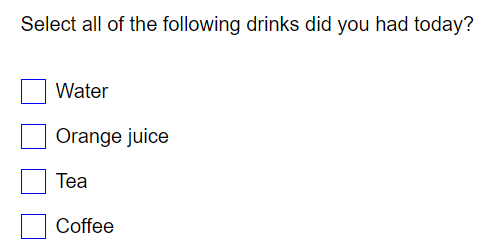
\includegraphics[width=.5\linewidth]{PsyToolkit/Figures/SurveyCheckbox.PNG}
        \label{fig:checkboxexample}
    \end{center}
    \begin{codeblock}{PsyToolkit code (top) and preview (bottom) for creating a simple question with checkbox options.}\label{code:psytoolkitquestion}\end{codeblock}
\end{tcolorbox}

Of course, when you are just starting out with PsyToolkit, the process of creating an entire survey with many different question types can seem a bit daunting.  Fortunately, PsyToolkit also offers an ``Easy" mode that can be especially helpful for beginners.  To enter easy mode, simply click the button labeled ``easy mode" just above the survey editor (see Figure \ref{fig:psytoolkiteasymode}). 

\mywrapfigure{PsyToolkit Easy Mode}{.5\linewidth}{PsyToolkit/Figures/PsytoolkitEasyMode.PNG}{Adding survey items is as simple as a few clicks using ``Easy Mode".}{fig:psytoolkiteasymode}
When in easy mode, the items in your survey are listed in a convenient table that includes links to enable direct editing of each item.  New items can be added by clicking the \button{+} button.  When you add a new item, you will first be presented with a list of available item types.  The decisions you make about the types of items you include will be based on the kind of data you wish to collect and the parameters you want to impose on the participant's responses.  For example, most surveys will include an item requesting the participant to indicate their gender.  One possibility would be to use a text line where the participant can enter whatever response they like using the keyboard. In this case, it will be up to you as the researcher to comb through the responses and group similar responses like ``male", ``Male", ``M", ``boy", or maybe even ``mail".  This could be a tedious and error-prone process, so a more appropriate choice when requesting the participant's gender might be to use the radio button type item with options for ``Male" and "Female", which would simplify data entry for the participant \emph{and} data analysis for the researcher.  In short, you should carefully consider how you select items for your survey.  You can add as many items to your survey as you like.

Of course, items are the most important part of your survey as they determine the kinds of information/data that are collected.  However, whenever collecting data from human participants, it is important to provide them with enough information about the study that they can make an informed decision about whether or not they would like to participate \emph{before} you start collecting data.  This kind of information that is required for \gls{informed consent} is also designated in the survey design page using the text fields available in the ``Survey intro screen and special options" section of the PsyToolkit survey generation page.  

If you are still in easy mode, you will first need to return to the regular mode by clicking the \button{regular overview} button (see Figure \ref{fig:psytoolkiteasymode}). Next, scroll down to the ``Survey intro screen and special options" section.  There you will find options governing the look and feel of your survey, an ``About this survey" section where you can enter information to be provided to the participant \emph{before} they begin the survey, an expandable ``Read more" section for additional information, and a ``Contact information" section where you can provide the participant with contact information for the \gls{principal investigator} (PI). Once you have entered all of this information (\emph{don't forget to click the \button{Click to save} button at the bottom!}), you are ready to compile and test your survey.

\subsubsection{Test Your Survey}
Before you deploy your survey you will, of course, want to test it out.  This requires that you first \gls{Compile} your survey for execution. If you are still in easy mode, you will first need to return to the regular mode by clicking the ``regular overview" button (see Figure \ref{fig:psytoolkiteasymode}) and take the following steps:

\begin{enumerate}
    \item Scroll down to the ``Compile/test survey" section and click the \button{compile} button (see Figure \ref{fig:psytoolkitcompilesurvey}).
\myfigure{Compile/test your survey}{PsyToolkit/Figures/PsytoolkitCompileSurvey.PNG}{Use the ``Compile" button to compile and test your survey.  You will get a message letting you know if there were errors or if it compiled correctly.}{fig:psytoolkitcompilesurvey}{\linewidth}{.76\linewidth}{.23\linewidth}
Note that if your survey does not compile correctly PsyToolkit is designed to give detailed feedback of how to fix errors. PsyToolkit will tell you which line of your script file the problem occurs in.  If you are having trouble getting your survey (or experiment) to compile, you may want to check the Problem solving \& Tips page at \weblink{https://www.psytoolkit.org/software/problemsolving.html}.

\item Once your survey has compiled successfully, scroll down to the ``Online/Offline survey status" section and select the option, ``Survey is online. For when you are still designing it." and then click the \button{Change survey status} button.
\myfigure{Compile/test your survey}{PsyToolkit/Figures/PsyToolkitTestStatus.PNG}{Use the ``Compile" button to compile and test your survey.  You will get a message letting you know if there were errors or if it compiled correctly.}{fig:psytoolkitteststatus}{\linewidth}{.76\linewidth}{.23\linewidth}

\item When the status has been changed, you will be provided with a \gls{URL} that can be copied into the address bar of your browser which will take you to the online survey (see Figure \ref{fig:psytoolkitteststatus}).
\end{enumerate}

When you follow the link to your survey, you will first see all of the information provided in the ``About this survey" section.  Once the button is clicked to start the survey, each of the items is presented one-by-one until all of the items have been answered (see Figure 

\subsubsection{Check the Survey Data}
All responses are automatically saved any time the survey is completed.  In order to view and/or download the data, simply scroll to the bottom of the page used to edit your survey in PsyToolkit and find the ``Prepare and download participant data" section.  Click the \button{Prepare datafiles for download} button.  Soon thereafter (after a couple of refreshes), a \button{download data in zip file} button will appear.  Click that button to download your data (see Figure \ref{fig:psytoolkitdownload}).

\mywrapfigure{PsyToolkit Data Download}{.5\linewidth}{PsyToolkit/Figures/PsyToolkitsurveydownload.PNG}{PsyToolkit Data Download}{fig:psytoolkitdownload}

The data files will be compressed into a single .zip file.  When you find the downloaded file, uncompress (i.e., unzip) it to your favorite location on your computer.  The unzipped folder will be called ``data" by default.  Inside, you will find a number of files, including a copy of the original survey script file in ``survey.txt", individual text files containing raw data from each of the participants separately, the participant's \gls{aggregate data} in ``data.csv" and ``data.xlsx" (two formats are provided for convenience), and aggregate data about the times/dates when the surveys were completed in ``data\_times.csv" and ``data\_times.xlsx". 

It may take some time to understand how your data are organized.  Although each row of the tabular output is dedicated to one of the participants, each of the item types has a slightly different data storage format.  For example, the ``radio" items only allow for one response to be selected, so the result is stored in a single column (see Figure \ref{fig:psytoolkitdataformat}).  The ``check" item types allow users to select multiple items, so each of the available responses is listed as a column and a \texttt{0} or a \texttt{1} is used to indicate the absence/presence of a check-mark for that item (see Figure \ref{fig:psytoolkitdataformat}).

\myfigure{Aggregate Survey Data}{PsyToolkit/Figures/PsyToolkitDataFormat.PNG}{Aggregate Survey Data.}{fig:psytoolkitdataformat}{\linewidth}{.82\linewidth}{.17\linewidth}

\subsubsection{Deploy Your Survey}
It is important that you inspect and understand the aggregated output from PsyToolkit \emph{before} you deploy your survey to participants. Imagine that, only after putting all the time and effort into designing a survey, coding it in PsyToolkit, and collecting data from participants, you find out that a critical piece of information is missing from your survey or that the data you collected aren't appropriate for the analysis you had in mind.  Although it can take some time, thorough testing can mean the difference between a successful and a failed research project. That said, once you have thoroughly tested your survey, it is a simple matter to deploy it for real data collection using the following steps.

\begin{enumerate}
    \item First, it is usually a good idea to clear the data recorded while testing. Scroll to the bottom of your survey's page in PsyToolkit and click the \button{delete participant data files} button.
    \item Next, scroll up to the ``Online/Offline survey status" section and select the ``Survey is online. For when real data collection is going on" option and then click the \button{change survey status} button.
\end{enumerate} 

%\begin{wrapfigure}{R}{0.35\textwidth}
\begin{wrapfigure}[16]{R}[0pt]{.35\textwidth}
\begin{tcolorbox}[width=\textwidth,colback=yellow!5!white,colframe=yellow!50!black,
  colbacktitle=yellow!75!black,title=Food For Thought,grow to right by=1cm]
  \emph{Even creating a simple survey requires creativity and critical thinking!}
  \tcblower
  When a researcher creates an instrument for their research like a survey or experiment, there are many different decisions that must be made along the way.  For example, if you decide to ask your participants to indicate their gender, do you use male/female radio buttons, a text box that will permit a free response, or a drop-down menu.  These decisions will impact the experience of participants as well as the format of the recorded data, which may later impact the researcher's approach to data analysis.  In short, survey and experiment design are important skills for any psychological scientist.
\end{tcolorbox}
\end{wrapfigure}
You will again be provided with a link to your active survey.  This link can be shared with anyone you would like to complete your survey (or even shared publicly).  The only difference now is that your survey cannot be modified until you again change its status in PsyToolkit.

\subsection{Create Your First Experiment}
In the previous section, we covered how to create and deploy a simple survey using PsyToolkit. In the following sections we will see how to create and deploy experiments. While both survey and experiment methods are important in data collection and both can be used to test hypotheses, experimental research involves the manipulation of an independent variable and measuring its effect on a dependent variable.  In the context of research in the psychological sciences, the dependent variables are commonly measures like reaction time, accuracy, and number of items remembered while the independent variables are typically physical properties of the experimental stimuli like color, shape, emotional valence, and duration of exposure. In the following tutorial we will cover the steps necessary to create a simple reaction time task using PsyToolkit.  More advanced examples and detailed information can be found in the online documentation at \weblinkT{https://www.psytoolkit.org/doc3.2.0/}{https://www.psytoolkit.org/doc3.2.0/}.

Before you get started programming your task, it is always a good idea to lay out a specific plan. In this example, the aim is to re-create the simple reaction time task from the Donders experiments described earlier.  Thus, the experiment will minimally consist of the following: \begin{itemize} \item Presentation of  a fixation point (used to direct the attention of the participant) \item Presentation of a target stimulus \item Detecting and recording response times \end{itemize}  Identifying all of the major components of a task can be made easier by developing a \gls{task schematic} (see Figure \ref{fig:schematic}).  The task schematic will often illustrate the experimental stimuli, highlight the major parameters of an experimental task such as the time between stimuli, called the \gls{inter-stimulus interval} (ISI), and show how responses were collected from participants.

Working from the task schematic in Figure \ref{fig:schematic}, we can see that programming this experiment will require  at least two visual stimuli that will be presented to the participant, the fixation cross and the target stimulus (a diamond shape in this case) and the collection of a response from the keyboard.  We will also need to define an ISI and and an \gls{inter-trial interval} (ITI; not shown in the schematic) which will determine how much time should elapse between the response to one stimulus and the appearance of the fixation cross indicating the impending appearance of the next stimulus.

\myfigure{Example of a Task Schematic}{PsyToolkit/Figures/schematic.PNG}{The task schematic makes explicit the parameters of an experiment and can serve as a planning tool during programming \emph{and} as a visual aid for readers at the time of publication.}{fig:schematic}{\linewidth}{.5\linewidth}{.45\linewidth}
Creating a task schematic before you begin programming an experiment can be a useful in that is provides a convenient visual reference when determining how to program your experiment and it can also serve as a visual aid for readers when the experiment is completed and you are presenting the results of your experiment. For now, the task schematic can be used to determine the stimuli that need to be created. 

\subsubsection{Creating the Stimuli}
After having planned out your experiment but before beginning the work of programming that experiment in PsyToolkit, it is prudent to create the experimental stimuli (i.e., images and sounds) that will be presented to participants.  For present purposes, we will focus on the two images that will be presented to participants in the simple reaction time task, namely the fixation cross and the diamond shape.

PsyToolkit works best with a particular type if image file called a bitmap that includes the file extension ``\texttt{.bmp/.gif/.png/.jpeg, etc.}".  Simple bitmap files can be created using many different applications, including some of those installed by default on most Windows and OSx operating systems.  For more complex images and/or for better control over the parameters of those images, you will need to use a commercial image editor like Adobe Photoshop\copyright or one of its free alternatives like the Gnu Image Manipulation Program (GIMP) or Inkscape. PsyToolkit's authors recommend the free image editing software called Inkscape.  You can download your own copy of Inkscape for Windows or OSx at \weblink{https://inkscape.org/}.

\mywrapfigure{Inkscape}{.5\linewidth}{PsyToolkit/Figures/inkscape.PNG}{Inkscape is a free image editor that can be used to generate the bitmap files for use with PsyToolkit.}{fig:inkscape}

Figure \ref{fig:inkscape} illustrates how the two images were created in Inkscape for this tutorial.  Note that while a blue background was used in the example task schematic, a black background was selected for the actual stimuli so that they could more easily match the default background screen color in a PsyToolkit experiment.  Also note that although the two images are illustrated in a single window, they were saved as two separate files, ``fixation.png" and ``target.png".  Once you have created the bitmaps for an experiment, these files must be uploaded to your experiment folder in PsyToolkit. Follow these steps to upload files to your experiment's page in PsyToolkit:
\begin{itemize}
    \item Click the \button{Choose files} button
    \item Find and select the file(s) on your computer and click \button{Open}.
    \item Click the blue \button{Save} button in PsyToolkit to complete the upload.
\end{itemize}
Files uploaded to an experiment can be viewed, deleted, and renamed by clicking the \button{view files} button.

\subsubsection{The Experiment Script}
Now that you have both a clear plan in place for developing your experimental protocol and you have created the stimuli you will be using, you are ready to begin writing the program that will be compiled and run using PsyToolkit. This program must be written using an experiment script, which is a set of instructions that will determine all aspects of your program including which stimulus files to use, when to present them, what data to collect, etc.  A minimal working example of a PsyToolkit experiment script is illustrated in the code block below. \emph{Note that any text following the ``\#" is an explanatory comment and will NOT be executed when the program is compiled!}

\begin{tcolorbox}[every float=\centering, drop shadow,     title=The Simple RT Experiment Script]
\begin{verbatim}
options
fullscreen                #run in full-screen mode

bitmaps
  fixation                #load fixation.png
  target                  #load target.png

task SimpleRTTask
  keys space              #listen to the "space" key
  delay 1500              #don't do anything for 1,500ms (ITI)
  show bitmap fixation    #show fixation.png 
  delay 1000              #don't do anything for 1000ms (ISI)
  clear -1                #clear the last image shown
  show bitmap target      #show bitmap.png 
  readkey 1 2000          #wait for spacebar press for no more than 2000ms
  set $rt RT              #set variable "rt" to value of RT
  save $rt                #save rt for this trial
  clear -1                #clear the last image shown
  
block SimpleRTBlock
  tasklist
  SimpleRTTask 50         #run the SimpleRTTask 50 times
  end
    \end{verbatim}
\tcblower
\begin{codeblock}{Minimal working example of a simple RT experiment script in PsyToolkit.}\label{code:experimentscript}\end{codeblock}
\end{tcolorbox}
Notice that the experiment script is divided into four sections, including (1) \texttt{options}, (2) \texttt{bitmaps}, (3) \texttt{task}, and (4) \texttt{block}.  Not all of these sections are strictly required for the experiment to run and there are other named sections that are not necessary for example.  Importantly, each of these sections helps to define a specific set of parameters that will govern the behavior of the experiment.  For example, the ``\texttt{fullscreen}" command in the \texttt{options} section tells PsyToolkit to run the experiment in full-screen mode on the participant's computer and the \texttt{bitmaps} section contains a list of names of the bitmap files that will be used. 

The \texttt{task} section can be thought of as the list of events that will occur on each trial of the experiment.  Recall that in the simple reaction time task, each trial consists of the presentation of a fixation cross, then the presentation of a diamond to which the participant is expected to respond by pressing a button. Of course, when writing a program to accomplish this, every last detail must be provided to PsyToolkit as a specific instruction.  As with any programming language, and as you can see from code block \thechapter.\ref{code:experimentscript}, there is a specific syntax required to give these instructions.  

Generally speaking, most instructions to PsyToolkit start with a keyword and are followed by one or more parameters.  For example, the keyword ``\texttt{keys}" instructs PsyToolkit to prepare to ``listen" for input from the keyboard and the subsequent parameter ``space" indicates that PsyToolkit need \emph{only} listen to input from the spacebar.  Similarly, the keyword ``\texttt{delay}" instructs PsyToolkit to pause the experiment and the parameter that follows provides PsyToolkit with a time-limit for the pause in milliseconds (ms).  In the present example, both the ITI and ISI are accomplished using the \texttt{delay} command.  We will cover some of the other commands later in this tutorial later.  

The final section of the experiment script is the \texttt{block} section.  Most experiments are complex and require the designation of more than one \texttt{task} section in the experiment script. The block section is where you would instruct PsyToolkit about how and in which order it should present participants with each task.  In the present example, we are using a very simple experiment with just a single \texttt{task} and so the \texttt{block} section simply sets up a task list with just one task (i.e., ``SimpleRTTask") and instructs PsyToolkit to repeat the simple reaction time task 50 times.

\subsubsection{Testing and Deploying Your Experiment}
Writing your own experiment script will almost always require several rounds of testing/troubleshooting before it is ready to be deployed.  Before you can test your experiment, you will need to both save and compile your experiment script in PsyToolkit.

To start testing your experiment, first press the \button{Save} button just below the experiment script.  Then, click the \button{compile} button in the next section, titled ``Compile and run".  If your experiment successfully compiles, you will see a message saying that it was successful and you will also see a \button{Run experiment} button that you can click to conduct a test-run of your experiment.  If the script does not compile successfully, you will see an error message informing you about the nature of the error.  Once that error has been addressed in the experiment script editor, you will need to re-save and re-compile the experiment script.
\myfigure{Compile and Run Section}{PsyToolkit/Figures/compile.png}{Illustration of the Compile and run section of PsyToolkit following a successful compiling of an experiment script.}{fig:compile}{\linewidth}{.8\linewidth}{.18\linewidth}

During testing, the results of your experiment are immediately available to you using the \button{View data} button that appears when the experiment has completed.  You also will have options to save the data for later analysis.  Once the experiment has been deployed for data collection, participants will NOT have the option to view their own data.

Deploying an experiment requires that it be embedded into a PsyToolkit survey. This is incredibly simple to do.  Recall that earlier in this tutorial, we created our first survey, titled ``My\_First\_Survey" with just two example questions (see Figure \ref{fig:psytoolkitsurvey}).  When a survey is open for editing, you can add just a few lines of code to embed your experiment. The code below illustrates how the ``SimpleRT\_Experiment" script can be embedded into ``My\_First\_Survey" just like any other survey element:
\begin{Verbatim}[xleftmargin=.5in]
l: SimpleRTExperiment   #just a label for the survey item
t: experiment           #the type of items is "experiment"
- SimpleRT_Experiment   #gives the name of the experiment to include
\end{Verbatim}

Once this item has been added to a PsyToolkit survey, all that is needed is to (1) save the survey, (2) re-compile the survey, and (3) make sure the survey status is set to one of the two ``online" options. After following these steps, you are ready to send out the link to your active survey and begin collecting data for your experiment.  

\subsection{Intermediate Experiment Generation}
\subsubsection{The Go\_No-Go Task}
In the previous section, we covered the basics of creating and deploying surveys and experiments with PsyToolkit.  The experiment used was a simple RT experiment just one target stimulus.  Of course the vast majority of experimental procedures in the psychological sciences involve much more complex procedures for manipulating and measuring an individual's behavioral performance.  For example, the second Donders procedure described above, called the ``GoNo-Go Task", involves the presentation of two different experimental stimuli, with the participant asked to first identify each stimulus and respond to only one of the two.  Unfortunately, generating such a task is more complex than simply adding a second stimulus (e.g., a square) image file and adding a new ``\texttt{show bitmap}" line to the experiment script.

To understand this, think for a minute about what you learned in the prior section.  The \texttt{task} section of experiment script is simply a list of instructions.  If you were to simply add a second stimulus presentation after the original diamond stimulus, then the experiment script would simply generate a perfectly predictable series of alternating stimuli (e.g., diamond $\rightarrow$ square $\rightarrow$ diamond, etc.).  The predictability of the sequence would preclude the need to do any identification since one could just learn to press the space bar on every other stimulus.  Thus, what is needed is a way to randomly select on each trial which of the two image files will be presented to participants.

There are several ways one could solve this problem.  One idea might be to have PsyToolkit choose a random number between 1 and 2 at the beginning of each trial and present the diamond image if the number is equal to 1 and the square image if the number is equal to 2. Another possibility is to create separate Go and NoGo ``\texttt{task}" sections in the experiment script and then list both of the tasks in the ``\texttt{block}" section of the experiment script.  As it turns out the latter option will be the simplest to implement in PsyToolkit.

\subsubsection{Random Selection of Tasks}
Before you start to incorporate random task selection into a Go/No-Go experiment, you should:
\begin{enumerate}\item Create the No-Go stimulus using your favorite image editor (I used the example of a square earlier).
\item Click the orange \button{copy} button in the set of ``Actions" options on the left side of the page.
\item Upload your No-Go stimulus image file.
\item Modify the experiment script to include a new ``NoGo" task and add that new task to the ``tasklist" in the ``block" section of the experiment script (see
Code block \ref{code:gonogo}). 
\end{enumerate}
\begin{tcolorbox}[every float=\centering, drop shadow,     title=The Go/No-Go Experiment Script]
\begin{center}<---SimpleRT experiment script snipped here--->\end{center}
\begin{verbatim}
[1]     task NoGo_Task
[2]       set $TrialType "NoGo"
[3]       keys space
[4]       delay 1500
[5]       show bitmap fixation
[6]       delay 1000
[7]       clear -1
[8]       show bitmap square
[9]       readkey 1 2000
[10]      set $rt RT
[11]      save $rt $TrialType
[12]      clear -1
[13]
[14]    block GoNoGo_Block
[15]      tasklist
[16]        SimpleRTTask 50
[17]        NoGo_Task 50
[18]      end
    \end{verbatim}
\tcblower
\begin{codeblock}{Illustration of the NoGo task and changes needed to "block" section of the Simple RT experiment script to incorporate the NoGo task into the Go/No-Go experiment script in PsyToolkit.}\label{code:gonogo}\end{codeblock}
\end{tcolorbox}

The first thing you should notice about the NoGo task in code block \thechapter.\ref{code:gonogo} is that it is almost exactly like the original ``SimpleRTTask" except that (1) the bitmap shown is ``square" instead of ``target" and (2) a variable called ``TrialType" has been set at the beginning of the NoGo task and is also saved along with the ``RT" variable.  The first difference is, of course, needed to change the shape of the stimulus.  The second difference will be clear later when we look at the stored data.  Note that there were several design options here.  For example, since participants are being asked to withhold their response when the square appears, it really isn't necessary to record the reaction time or even set up the ``keypress" listener at all.  However, recording erroneous responses to the presentation of the square could potentially be informative.  For example, if a participant presses the space bar whenever any of the two stimuli appear, it could be that they either did not understand or were not following the instructions.

The second change to notice in this experiment script is the simple addition of the ``NoGo\_Task" to the list of tasks in the ``\texttt{block}" section of the script, with 50 repeats (i.e., trials) designated for each task.  Although it may not be intuitive how this produces a random series of trials, it turns out that the default behavior of PsyToolkit is to pool all of the 100 ($50x2$) trials inside the \texttt{tasklist} and then randomly draw from those 100 trials without replacement.  Once you have completed the Go/No-Go experiment script, be sure to save and compile it as well as add a corresponding ``experiment" type item to your survey just like you did for the Simple RT experiment script.

\subsection{Retrieving Experiment Data from PsyToolkit}
Although we briefly covered the way data is stored by PsyToolkit in the context of survey responses.  It is important to also understand how data collected via an experiment are stored for analysis.  Just as you did earlier, click the \button{Prepare datafiles for download} button, then click the \button{Download data in zip file} button to get a copy of the data on your computer.

\myfigure{PsyToolkit Data Files}{PsyToolkit/Figures/datafiles.png}{Illustration of the way files are stored and named by PsyToolkit during data collection.}{fig:datafiles}{\linewidth}{.8\linewidth}{.17\linewidth}
The downloaded files will look very similar to those reviewed earlier.  There will be survey data files in \texttt{.csv}, \texttt{.xlsx}, and \texttt{.txt} formats.  You should also see, however, one or more separate text (\texttt{.txt}) files containing the data saved for the Go/No-Go experiment for each participant.  These files will always start with the name of the experiment and the date, and end with a string of seemingly random characters.  This random string of characters will be constant across participants.  In other words you will see matching  random strings in the survey and experiment data files as well as the aggregate data.

\mywrapfigure{PsyToolkit Experiment Data Files}{.35\linewidth}{PsyToolkit/Figures/expdata.png}{Inkscape is a free image editor that can be used to generate the bitmap files for use with PsyToolkit.}{fig:expdata}
For present purposes, the most important data files are the text (\texttt{.txt}) connected to the experiment.  These files can easily be opened in most spreadsheet software like Microsoft Excel and Google Sheets. When you open  files for PsyToolkit experiments, each row of the data represents a single trial of the experiment and any variables stored on each trial are represented by columns.  An example of the data file saved during the Go/No-Go task described above is presented in Figure \ref{fig:expdata}. Notice that the first entry in each row is a measure of the RT on that trial and that the No-Go trials are each denoted by the text ``NoGo" as the second entry in each row.

Of course, this was a minimal working example and you, as the experimenter (and programmer), have complete control over how the experiment is designed and even how the output is stored in some cases.  For example, recall from the code presented in Code block \thechapter.\ref{code:gonogo} that we added the \$TrialType variable to the No-Go task so as to be able to discriminate those trials in the output file.  It would be trivial to do the same for the task governing the Go trials so as to include a ``Go" label in the second column on those trials. You may also notice that when the participant correctly withheld their response on No-Go trials, a value of 2000 was recorded for the RT on that trial.  Hopefully you can reason that this value was entered because that was the time limit established in the experiment script for making a response. Although extremely unlikely, \clearpage \noindent it is possible for a participant to press the space bar at exactly 2000 milliseconds and such trials would be impossible to distinguish in the data as it is presently formatted.  This and many other aspects of the program are under the control of the experimenter in PsyToolkit, but do require more advanced knowledge of the scripting language.  

\subsection{Advanced Experiment Generation}
One could easily devote an entire course to learning the scripting language used by PsyToolkit.  Thus far, we have just scratched the surface of its capabilities.  Even the most intuitive GUIs for developing experiments require some knowledge of coding in their native languages in order to implement more complex experimental designs and the same is true for PsyToolkit.  Some common examples of the ways in which experiments become a little more difficult to implement are when the researcher would like to introduce randomness, when there are many experimental conditions (e.g., factorial designs), and when the researcher would like to implement conditional execution (e.g., display ``correct" \emph(ONLY) if the participant makes a correct response).

\subsubsection{Introducing Randomness}
When the hallmark of a good experiment is strict \emph{control} of the variables, it may seem odd to be discussing how to add randomness to an experiment.  However, there are a number of conditions under which randomness is actually used as a form of control over potential \gls{extraneous variables}.  In fact we already touched on this issue in the previous section.  Recall that in the sample Go/No-Go it was suggested that it would be a bad idea to include presentation of the two stimuli in the same ``task" section.  The reason for this was that if the sequence of stimuli was perfectly predictable, participants would not need to identify the stimuli at all since they could simply anticipate pressing the button every other time the computer screen illuminated. In this case, the participants ability to anticipate target stimuli is an extraneous variable that could have a significant impact on the dependent variable of RT.  In order to control this extraneous variable, our solution was to create two separate ``tasks" in the experiment script (one for each stimulus) and randomize the order of presentation in the ``block" section.

\mywrapfigure{Constant vs. Random ISI}{.7\linewidth}{PsyToolkit/Figures/AnticipationRT.png}{Inkscape is a free image editor that can be used to generate the bitmap files for use with PsyToolkit.}{fig:anticipationRT}
Another example of when randomness can help to control extraneous variables like participant anticipation is in the definition of experiment parameters like the ISI and ITI. For example, you may have noticed when testing the simple reaction time experiment above, that with the target stimulus appearing after the fixation cross at a consistent, 1 second, ISI it quickly becomes easy to anticipate the appearance of the target stimulus.  In fact, if you were to plot your reaction times over trials, you would see these  anticipatory benefits in the form of decreased RTs.  Figure \ref{fig:anticipationRT} illustrates this effect using RTs recorded using the simple RT task described above.  When participants complete the task with a constant, 1000ms ISI between the fixation cross and the target stimulus, there is a clear benefit of about 100ms that is reached by around the 20th trial.  Figure \ref{fig:anticipationRT} also illustrates how the introduction of randomness can control for the effects of anticipation.  When the simple RT task is completed with a random ISI between 800ms and 1200ms, the decrease in RT seen at the beginning of the experiment is entirely absent from the data. 

Adding randomness to an experiment is quite simple in PsyToolkit using the keyword ``\texttt{random}".  As with most other keywords, \texttt{random} must be followed by parameters that govern its behavior. Several examples of the use of the \texttt{random} keyword are provided below:
\begin{center}
\begin{tabular}{ l l l}
    Return a random value between 1 and 10 &= & \texttt{random 1 10}\\
    Return a random value between 2 and 100 in steps &= & \texttt{random 2 100 2}\\
    Return a random value from specific set of values &= & \texttt{random from 12 98 105 34}\\
    Return a random word from a list &= & \texttt{random from ``A" ``An" ``Are"}\\
\end{tabular}
\end{center}

Each of the expressions above returns a value that is typically assigned to a variable using the ``\texttt{set}" keyword.  A \gls{variable} in programming is like a container for information that can later be referenced or manipulated.  In PsyToolkit variable names are preceded by the dollar sign (\$) or the amperstand (\&). For example, a variable named ``ISI" with a stored value of 1000 could be created in PsyToolkit with either of the following lines:
\begin{Verbatim}[xleftmargin=2.5in]
    set $ISI 1000
         or
    set &ISI 1000
\end{Verbatim}

In either case, \$ISI or \&ISI is a container for the value 1000.  The difference between the two instances is that \&ISI is a \gls{global variable} and \$ISI is a \gls{local variable}.  Global variables are ``set" in the \texttt{options} section of an experiment script and can be used anywhere within the experiment script.  Local variables are ``set" within a \texttt{task} section of the experiment script and can \emph{only} be used within the task in which they are defined. For now, we will focus on the local variable \$ISI. The advantage of creating a constant variable like this might not be immediately obvious, but imagine that you've programmed a complex task using hundreds of lines of commands in which you have explicitly set the value of a delay interval to 1000ms in 250 separate places in the program.  Now imagine that you decide that you need to use a value of 1200 instead of 1000.  Without using a variable, this change would require you to manually find and change all 250 instances of the delay value.  Alternatively, by setting an \$ISI variable equal to 1000 at the beginning of the \texttt{task} script and then referring to that variable at each of the 250 instances, changing all of the delay times to 1200 would require \emph{only} a single change to the definition of the \$ISI variable at the top of the script.

Creating a variable that is assigned a random value is as simple as combining the \texttt{set} and \texttt{random} keywords.  For example, the following line would create an \$ISI variable with a randomly selected value between 800ms and 1200ms:
\begin{Verbatim}[xleftmargin=2in]
    set $ISI random 800 1200
\end{Verbatim}
Finally, implementation of the random delay interval for the ISI in a PsyToolkit experiment script is as simple as referencing the \$ISI variable when specifying the duration parameter of the \texttt{delay} keyword. (see lines 3 and 6 of code block \thechapter.\ref{code:randomisi}).

\begin{tcolorbox}[every float=\centering, drop shadow,     title=The Go/No-Go Experiment Script]
\begin{center}<---SimpleRT experiment script snipped here--->\end{center}
\begin{Verbatim}
[1]    task NoGo_Task
[2]      set $TrialType "NoGo"
[3]      set $ISI random 800 1200
[4]      keys space
[5]      show bitmap fixation
[6]      delay $ISI
[7]      clear -1
[8]      show bitmap square
[9]      readkey 1 2000
[10]     set $rt RT
[11]     save $rt $TrialType
[12]     clear -1
[13]
[14]    block GoNoGo_Block
[15]      tasklist
[16]       SimpleRTTask 50
[17]       NoGo_Task 50
[18]      end
    \end{Verbatim}
\tcblower
\begin{codeblock}{Example of using a random number to define the duration of the ISI in the NoGo task }\label{code:randomisi}\end{codeblock}
\end{tcolorbox}

\subsubsection{PsyToolkit Tables}
In the Go/No-Go experiment script covered earlier in this chapter, we used two separate \texttt{task} sections to create the two conditions of the experiment; one presenting participants with a diamond and expecting a press of the space bar, and the other presenting a square to which participants were expected to withhold their response.  This was a functional solution meant to simplify this introduction to PsyToolkit, but it is \emph{not} the best solution and would not likely work for most experimental designs.

The recommended method for defining the separate conditions of a task in PsyToolkit is by creating a ``\texttt{table}".  The \texttt{table} section of an experiment script defines a table with rows and columns. Each row of the table contains the parameters of the task that will define your trial types. Each time a table is being used in a task, one of its rows is chosen at random. Columns can be referenced using the @ sign. For example, ``@2" in an experiment script refers to the contents of the second column in whichever row was chosen for a given task trial. Users can specify how table lines are selected in the ``\texttt{block}" section of the experiment script (default=random).

In order to demonstrate the use of tables, let's consider how they might be used to re-create the third of Donders' reaction time tasks, the Choice Reaction Time task (see Figure \ref{fig:donders}).  Recall that the Choice RT Task involves presenting participants with two different stimuli (one at a time) and asking them to make one of two potential responses that depends on the identity of that stimulus.  By comparison with the Go/No-Go task created earlier, the only major change is that there will need to be two different response options.  Thus, the parameters of the Choice RT task that will change on each trial include the image file presented, and the response expected from the participant, defining the two experimental conditions. These parameters can easily be defined in a \texttt{table} like the one below.

\begin{Verbatim}[xleftmargin=2in]
table My_First_Table
   diamond  1  "Diamond"
   square   2  "Square"
\end{Verbatim}

In the example above, the first line simply denotes that what follows will define a ``\texttt{table}" section and gives this \texttt{table} the name ``\texttt{My\_First\_Table}".  The 2 subsequent lines define the parameters of each of the two conditions in the experiment, starting with the name of the bitmap file that will be presented (\texttt{diamond} or \texttt{square}), followed by the correct response for that trial (1 or 2), followed by a text label that will be used to identify the trial type in the output file ("Diamond" or "Square").

Once the table has been defined, it can be used inside the \texttt{task} section of the experiment script.  This is illustrated in the full working example illustrated in code block \thechapter.\ref{code:choiceRT}, which illustrates all of the concepts covered thus far, including the use of tables to define experimental conditions and setting up a random ISI.  One aspect of using tables to indicate correct responses that can be confusing for some new to PsyToolkit is that when more than one key is listed after the ``\texttt{keys}" command (see line 16 of code block \thechapter.\ref{code:choiceRT}), the parameter passed to ``\texttt{readkey}" (see line 21 of code block \thechapter.\ref{code:choiceRT}) is the number that corresponds with the serial position of the correct key in the ``\texttt{keys}" list.  For example, looking at the script in code block \thechapter.\ref{code:choiceRT}, if the second row of ``\texttt{My\_First\_Table}" is selected on any given trial, then line 21, ``\texttt{readkey @2 2000}", will cause PsyToolkit to read from keys \texttt{f} and \texttt{j} for 2000ms and consider the \texttt{j} key to be the correct response. This is because \texttt{@2} will refer to the second column of the table and the value in the second column of the second row is 2.  Line 16, ``\texttt{keys f j}", designates the set of appropriate keys and the key in position \#2 is \texttt{j}.    

\begin{tcolorbox}[every float=\centering, drop shadow,     title=The Choice RT Experiment Script]
\begin{Verbatim}
[1]    options
[2]      fullscreen                   #run in full-screen mode
[3]
[4]    bitmaps
[5]      fixation                     #load bitmap files
[6]      diamond
[7]      square
[8]
[9]    table My_First_Table           #create a table
[10]     diamond  1  "Diamond"        #define condition 1
[11]     square   2  "Square"         #define condition 2
[12]   
[13]   task ChoiceRT_Task             #create the choice RT task
[14]     table My_First_Table         #use My_First_Table in this task
[15]     set $ISI random 800 1200     #set a random ISI
[16]     keys f j                     #designate response keys
[17]     show bitmap fixation         #show bitmap named "fixation"
[18]     delay $ISI                   #delay for ISI duration
[19]     clear -1                     #clear the last shown bitmap
[20]     show bitmap @1               #show bitmap named in column 1 of table
[21]     readkey @2 2000              #correct key is in column 2 of table
[22]     set $rt RT                   #record RT in variable $rt
[23]     set $status STATUS           #record STATUS in variable $status
[24]     save @3 $rt $status          #save column 3 label, $rt and $status
[25]     clear -1                     #clear the last shown image
[26]     delay 1500                   #delay 1500ms at end of trial
[27]
[28]    block ChoiceRT_Block          #set up a block of trials
[29]      tasklist                    #set up list of tasks            
[30]       ChoiceRT_Task              #draw trials from ChoiceRT_Task
[31]      end
    \end{Verbatim}
\tcblower
\begin{codeblock}{Annotated example of a Choice RT task using randomness and a table to define conditions.}\label{code:choiceRT}\end{codeblock}
\end{tcolorbox}

One other notable addition to this latest example of an experiment script is that in addition to recording the RT from \texttt{readkey} in the variable \$rt, line \#23 records the STATUS from \texttt{readkey}.  When the \texttt{readkey} function records that one of the listed keys has been pressed, the STATUS will be set to CORRECT (numerical value 1) if the key designated in the second parameter of the \texttt{readkey} function was pressed. Otherwise, if the participant presses the wrong key, it will be set to WRONG (numerical value 2), and if there is no response at all within the designated time limit, the STATUS code will be TIMEOUT (numerical value 3).  Adding the \$status variable will facilitate the identification of these different categories of responses in the analysis of the data saved by this experiment script, which will look similar to the example in Table \ref{tab:choicedata}.
\begin{center}
\begin{table}[h]
\begin{tabular}{ l l l}
    Square & 744 & 1\\
    Square & 1422 & 2\\
    Diamond & 748 & 2\\
    Square & 2000 & 3\\
    Diamond & 843 & 1\\
    %\vdots & \vdots & \vdots\\
\end{tabular}
\caption{\label{tab:choicedata}Sample output data from the Choice RT experiment. The columnar data include: (1) name of the image file presented, (2) RT, and (3) the \texttt{readkey} STATUS (i.e., \$status).}
\end{table}
\end{center}

\subsubsection{Conditional Execution}
At this point, you should have all of the knowledge needed to develop a wide range of experiments using PsyToolkit.  However, you may have noticed that all of the experiment scripts developed so far are completely determinate (aside from the order in which stimuli are presented).  That is, once started, the experiment just runs through from beginning to end, even if the participant were to fall asleep at the computer!  While this may be sufficient in some limited circumstances, it is very often the case the behavior of the experiment will need to change depending on the circumstances of each trial including, but not limited to, the behavior of the participant.

In programming, this kind of dynamic behavior of a program is called \gls{conditional execution}, when some instructions in the experiment script are executed \emph{only} if a test condition is determined to be true.  Such behavior is most commonly accomplished in PsyToolkit using what is called an ``\emph{if}" statement, which takes the general form below where the condition is a logical statement that is either true or false.

\begin{Verbatim}[xleftmargin=1.5in]
    if CONDITION
      CODE EXECUTED IF CONDITION IS TRUE
    fi
\end{Verbatim}

At the heart of the if statement is the logical condition that will be evaluated when the experiment script is run.  These logical statements are created using logical operators as seen in the examples in Table \ref{tab:logic}.
\begin{center}
\begin{table}[h]
\begin{tabular}{ c c c c}
    \textbf{Operator} &  \textbf{Definition} & \textbf{Example} & \textbf{Result}\\
    \hline
    \hline
    \texttt{==} & is equal to & 100 == 102 & \texttt{FALSE}\\
    \texttt{!=} & is not equal to & 100 != 102 & \texttt{TRUE}\\
    \texttt{>} & greater than & 100 > 102 & \texttt{FALSE}\\
    \texttt{<} & less than & 100 < 102 & \texttt{TRUE}\\
    %\vdots & \vdots & \vdots\\
\end{tabular}
\caption{\label{tab:logic}Several examples of logical statements, their interpretation, and their result.}
\end{table}
\end{center}

Although each of the examples in Table \ref{tab:logic} uses explicit numerical values in the logical expression, logical expressions can also involve variable names in your experiment script.  Combining what we've learned about the format of an if statement in PsyToolkit, the construction of logical statements using logical operators, and the use of variables in PsyToolkit, let's look at some examples (below) of several useful if statements that could be used in an actual experiment script.

One of the most common uses of conditional execution is to control the feedback that is given to participants after they respond to a stimulus.  For example, the researcher may wish to show the participant a bitmap with the word ``correct" only if the response just executed was the correct response.  Using what you have learned so far, that behavior could be implemented in the Choice RT experiment script (see Code block \ref{code:choiceRT}) by inserting the code below into the experiment script after the response has been made and the target stimulus cleared from the screen (line \#25).
\begin{Verbatim}[xleftmargin=2.1in]
    if $status == 1
      show bitmap correct
    fi
\end{Verbatim}

One could use a similar if statement to display a bitmap with the word, ``incorrect" when the participant makes an error by simply changing the logical statement to \texttt{if \$status == 2} and changing the name of the bitmap file shown. It also turns out that there is an alternative approach that is even easier since all that is required here is to display some text to the participant.  Rather than creating separate bitmaps for ``correct" and/or ``incorrect", the \texttt{show text} command, which simply displays text to the participant, may come in useful here.  For example, the command:\\
\begin{center}\texttt{show text "Hello World"}\end{center}
would display the text, ``Hello World" to the center of the monitor.

Conditional expressions can also be combined using the logical operators \texttt{\&\&} (``and") and \texttt{||} (``or").  For example, what if you wanted your experiment script to show a special message like ``Slow Down", but only if the participant made an incorrect response \emph{AND} the response time was impossibly fast (e.g., less than 100ms).  The simplest way to accomplish this goal would be to use a single if statement with a compound conditional expression and the \texttt{show text} command as illustrated below:
\begin{Verbatim}[xleftmargin=2in]
    if $status == 2 && $rt < 100
      show text "Slow Down!"
    fi
\end{Verbatim}

\subsubsection{Tying Up the Loose Ends}
In this chapter, you have learned how to create surveys and experiments using PsyToolkit.  By now you should be able to create and deploy an experiment that involves the collection of RT and accuracy data, random selection of stimuli, randomization of parameters like ISI and ITI, and even conditional execution to display custom feedback messages.  However, even if you were to follow all of the instructions in this chapter to the letter, would the example scripts be ready for deployment?  Probably not!  You, as the programmer, did not need to be instructed about how to respond to the stimuli presented, but a naive participant would have no idea what to do when that first stimulus appeared on the screen.

Incorporating task instructions into an experiment is important both because it provides participants with instructions and because it ensures standardization of instructions across all participants.  Instructions screens can be created and presented just like any other bitmap you would use in your program.  In other words, you already know everything you need to know in order to set up one or more instructions screens at the beginning of an experiment.  Fortunately, however, there are some dedicated commands in PsyToolkit that make the process of presenting ``messages" to participants exceedingly simple.

The ``\texttt{message}" and ``\texttt{pager}" commands can be used for instructions and/or end screens.  These commands can be conveniently inserted into the the ``\texttt{block}" section of the experiment script (see example below).  
\begin{Verbatim}[xleftmargin=2in]
block Myblock
  message MyInstructionBitmap
  tasklist
    ChoiceRT_Task 100
  end
  message ThankYouBitmap
\end{Verbatim}
By default, the \texttt{message} command will present the named bitmap image and leave it on-screen until the participant presses the space bar key.  This kind of self-pacing of the instructions is often desired to ensure that all participants have adequate time to read and understand the instructions.

In the event that several instructions screens are required, one could simply use more than one \texttt{message} command, however a drawback is that participants can't go backward after they have moved from one screen to the next.  This limitation is solved with the \texttt{pager} command, which accepts a list of bitmaps and allows participants to scroll through that list using the arrow keys (see example below).
\begin{Verbatim}[xleftmargin=2in]
block Myblock
  pager MyInstruction1 MyInstruction2 MyInstruction3
  tasklist
    ChoiceRT_Task 100
  end
  message ThankYouBitmap
\end{Verbatim}

Note that, by default, the \texttt{pager} function requires the participant to press the ``q" to proceed beyond the final bitmap to begin the experiment.  Thus, the text of your final bitmap should instruct participants as such.  That said, having finalized your experiment with a clear set of instructions, it is now ready to be added to a survey and deployed for data collection.
\clearpage

\begin{tcolorbox}[width=\textwidth,colback=blue!5!white,colframe=blue!50!black,
  colbacktitle=blue!75!black,title=\Huge{PsyToolkit Assignment}]
  In a single file, re-create Donders' Simple RT, Go/No-Go, and Choice RT tasks using PsyToolkit.  Your experiment must meet the following criteria:
  \begin{enumerate}
      \item First slide shows your full name
      \item Includes one or more instructions pages at the start of each of the three RT tasks
      \item Includes 50 trials per RT task
      \item Includes Correct/Incorrect feedback after response on each trial (No response = incorrect)
      \item Thank you screen at end of the experiment
      \item Output data file contains four columns in the following order: [1] RT task name (``Sim'', ``GNG'', or ``CH''), [2] trial type (``Target'' or ``NonTarget''), [3] Accuracy (``0'' or ``1''), and [4] Reaction time. 
  \end{enumerate}
  \tcblower
  Illustration of correct output format (\emph{note that yours will not include column names}):
  \begin{center}
  \begin{tabular}{c c c c}
  \emph{Task Name} & \emph{Trial Type} & \emph{Accuracy} & \emph{RT}\\
  \hline
  \hline
  Sim & Target & 1 & 458\\
  Sim & Target & 0 & 173\\
  Sim & Target & 1 & 634\\
  . & . & . & .\\
  . & . & . & .\\
  . & . & . & .\\
  GNG & Target & 1 & 682\\
  GNG & NonTarget & 1 & 591\\
  GNG & NonTarget & 0 & 614\\
  . & . & . & .\\
  . & . & . & .\\
  . & . & . & .\\
  CH & Target & 1 & 782\\
  CH & Target & 1 & 791\\
  CH & Target & 0 & 714\\
  \end{tabular}
  \end{center}
\end{tcolorbox}
\printglossary[type=datacollection,style=twocolumn]
%\printglossary
%\glsresetall
\newpage
\bibliographystyle{apalike}
\renewcommand{\bibname}{References}
\bibliography{bibliography}
